\subsection{SharedLib}
I de følgende afsnit vil der kunne læses om unittests for \gls{SL}.\\\\


\textbf{Introduktion}\\
\gls{SL} har været testet iterativt som en del af projektets sprints, hvilket har betydet at der gennemgående har været minimale ændringer i eksisterende kode. I de følgende afsnit vil der blive beskrevet yderligere hvordan unittesting har fungeret og hvilke værktøjer der har været brugt.\\

\textbf{Testdetaljer}\\
I \gls{SL} er der en total testcoverage på \textit{96 procent} og dette er fordelt på \textit{249} unittests. Størstedelen af disse, \textit{177}, ligger i CmdMarshallers som også er der det meste af \gls{SL}'s logik ligger. Tests er lavet ved hjælp af NUnit~\cite{NUnit} og NSubstitute~\cite{NSubstitute} og coverage analyse er foretaget med dotCover~\cite{dotCover}. Det hele er samtidig blevet bygget løbende på en continuous integration server, mere specifikt Jenkins.~\cite{Jenkins}.

\begin{figure}[H]
	\centering
	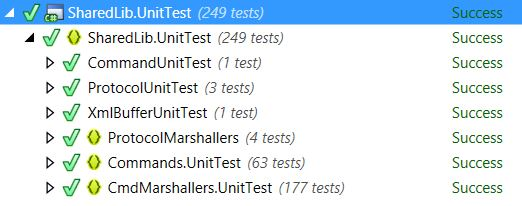
\includegraphics[width=0.60\textwidth]{Test/SharedLib/UnitTests/Unittests.jpg}
	\caption{Antal unittests for SharedLib}
	\label{fig:antalunitSL}
\end{figure}

\begin{figure}[H]
	\centering
	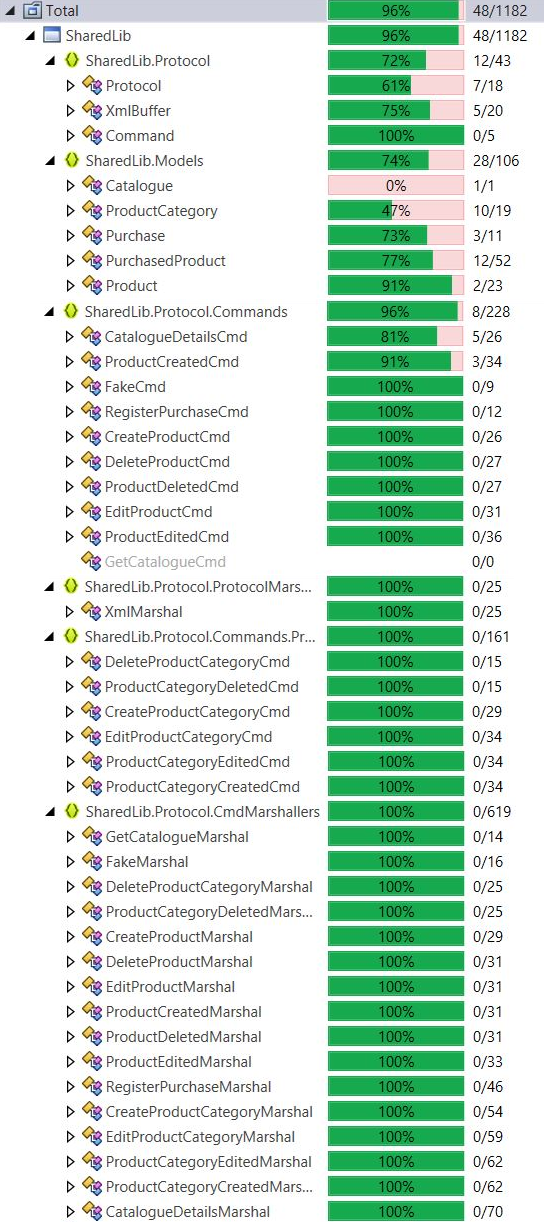
\includegraphics[width=0.60\textwidth]{Test/SharedLib/UnitTests/UCoverUlt.png}
	\caption{Testcoverage for SharedLib}
	\label{fig:coverSL}
\end{figure}


\newpage
\textbf{Beskrivelse af tests}\\
I \gls{SL} har størstedelen af unittests som det ses på figur \ref{fig:antalunitSL} omhandlet marshallerne\footnote{Marshallers er nærmere beskrevet i afsnit \ref{MARSHALLER} på side \pageref{MARSHALLER}}, da disse klart indeholder mest logik og størst kompleksitet. Marshallernes Encode/Decode funktioner, gjorde at der skulle en del tests til at dække grænseværdierne. derfor endte dette ud i et utroligt højt antal af tests. Enkelte funktioner i forskellige model klasser samt Sockets\footnote{Sockets klasserne: CommandListener og SocketConnection er nærmere beskrevet i afsnit \ref{SOCKET} på side \pageref{SOCKET}} klasserne blev ikke testet i dette afsnit da disse blev brugt i forbindelse med andre systemer og er derfor testet andetsteds.